The multiple asset test cases are designed to test the loss aggregation functions of the event-based risk calculator, such as:

\begin{itemize}
\item portfolio loss computation for a given ground motion field
\item calculation of portfolio loss exceedance curves
\end{itemize}

The major differences from the single asset calculations that need to be considered in the multiple asset tests include the possibility of having spatially-correlated ground motion fields and correlated vulnerability models for different assets of the same taxonomy.

% ---------------------------------------------------------------------------
\subsubsection{Case 6a}
The purpose of this case is to test the basic elements of an event based risk calculation involving multiple assets, such as computation of the individual asset loss curves, the portfolio loss exceedance curve, average asset losses, and the average portfolio loss.

The list of assets and their taxonomies are shown in Table~\ref{tab:assets-tax1}, and Table~\ref{tab:vf-ln-tax1-zcov} shows the mean loss ratios and corresponding coefficients of variation in the vulnerability function used in this test case.

As in previous cases, ground motion fields are generated for each of the ruptures generated in the 100,000 stochastic event sets. These ground motion fields take into consideration both the inter-event and intra-event variability in the ground motion. The ground motion prediction equation used is Boore and Atkinson (2008), and the Jayaram and Baker (2009) model for spatial correlation of ground motion values is applied. These ground motion fields are also used for the corresponding calculation in Julia.

Since there is no variability in the loss ratio, calculation of the loss ratios is straightforward in this case. The loss tables for each of the seven assets in the portfolio is compiled in the same manner as described in the single asset Case~1a. Since the coefficients of variation in the vulnerability function are all zero, the lognormal distribution devolves into the degenerate distribution. Thus, the sampled loss ratio at a particular ground motion intensity level is always equal to the mean loss ratio at that intensity level obtained through interpolation. Since there is no random sampling of the loss ratios in this case, we should expect to find the results from OpenQuake and Julia to be exactly identical.

The portfolio loss curve calculated using the implementation of the calculator in Julia is compared with that produced by OpenQuake in Figure~\ref{fig:lc-ebr-6a}.

\begin{figure}[htbp]
\centering
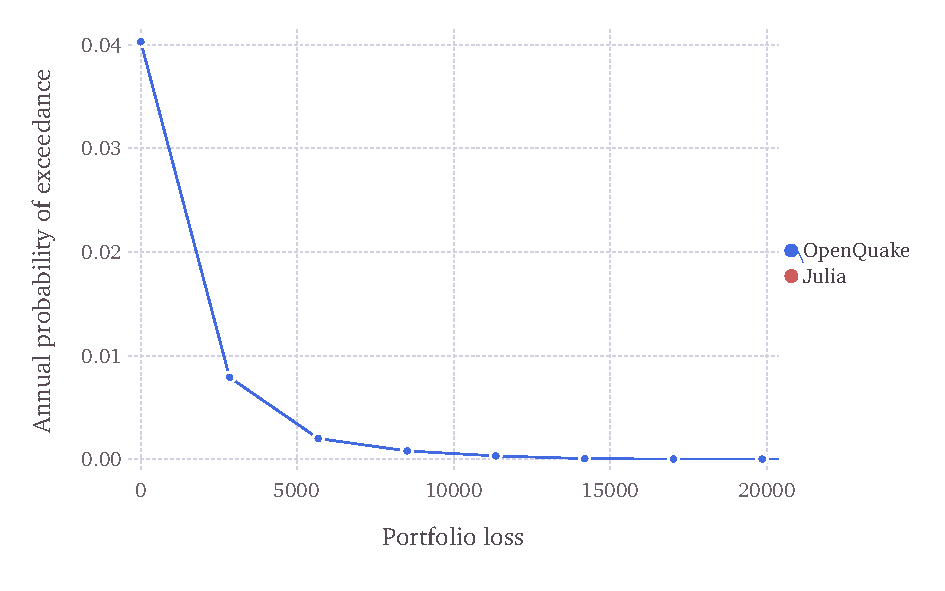
\includegraphics[width=12cm]{qareport/figures/fig-lc-ebr-6a}
\caption{Portfolio loss curve comparison for event based risk test case 6a}
\label{fig:lc-ebr-6a}
\end{figure}
\begin{table}[htbp]

\centering
\begin{tabular}{ l r r r }

\hline
\rowcolor{anti-flashwhite}
\bf{Result} & \bf{Julia} & \bf{OpenQuake} & \bf{Difference}\\
\hline

\hline
\end{tabular}

\caption{Results for event based risk test case 6a}
\label{tab:result-ebr-6a}
\end{table}
Table \ref{tab:result-ebr-6a} shows the comparison of the OpenQuake result for average asset losses and average portfolio loss with the expected result.

% ---------------------------------------------------------------------------
\subsubsection{Case 6b}
This case involving multiple assets is designed to test of the computation of the individual asset loss curves, the portfolio loss exceedance curve, average asset losses, and the average portfolio loss, when the vulnerability models of different assets of the same taxonomy are treated as uncorrelated. In OpenQuake, this can be specified in the job configuration file, by setting the value of the parameter `asset\_correlation' to zero.

The list of assets and their taxonomies are shown in Table~\ref{tab:assets-tax1}. Table~\ref{tab:vf-ln-tax3-zcov} shows the mean loss ratios and corresponding coefficients of variation in the vulnerability function used in this test case.

Ground motion fields are generated for each of the ruptures generated in the 100,000 stochastic event sets. These ground motion fields take into consideration both the inter-event and intra-event variability in the ground motion. The ground motion prediction equation used is Boore and Atkinson (2008), and the Jayaram and Baker (2009) model for spatial correlation of ground motion values is applied. These ground motion fields are also used for the corresponding calculation in Julia.

Since the sampled loss ratios conditional on a given ground motion field for different assets of the same taxonomy are assumed to be uncorrelated in this case, a loss ratio is sampled independently for each asset from the univariate lognormal distribution for that asset for each ground motion field.

The portfolio loss curve calculated using the implementation of the calculator in Julia is compared with that produced by OpenQuake in Figure~\ref{fig:lc-ebr-6b}. Only the aggregated results for the portfolio are shown here for brevity.

\begin{figure}[htbp]
\centering
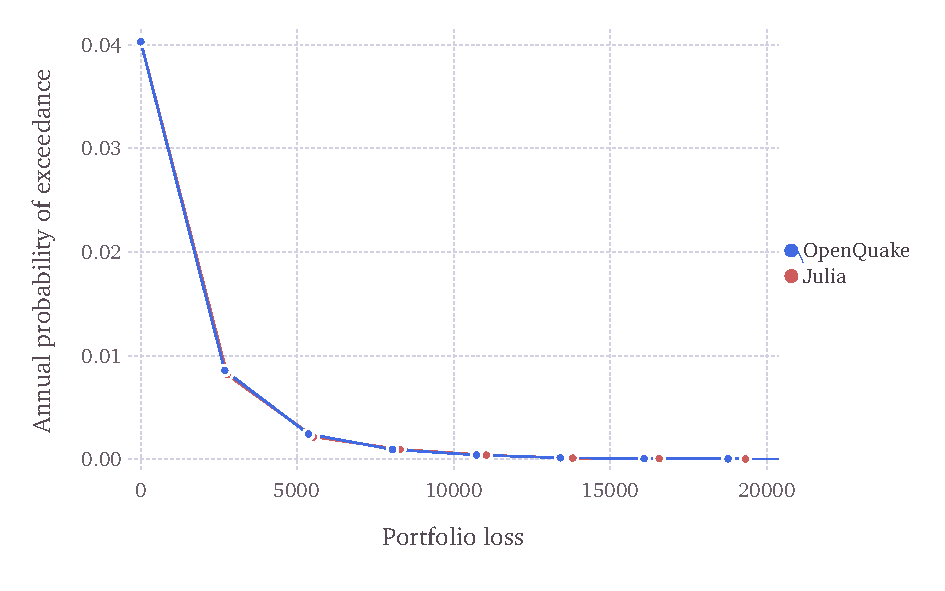
\includegraphics[width=12cm]{qareport/figures/fig-lc-ebr-6b}
\caption{Portfolio loss curve comparison for event based risk test case 6b}
\label{fig:lc-ebr-6b}
\end{figure}
\begin{table}[htbp]

\centering
\begin{tabular}{ l l r r r }

\hline
\rowcolor{anti-flashwhite}
\bf{Asset} & \bf{Result} & \bf{Julia} & \bf{OpenQuake} & \bf{Difference}\\
\hline
Portfolio & Average loss & 88.48 & 87.89 & 0.66\% \\
\hline
\end{tabular}

\caption{Results for event based risk test case 6b}
\label{tab:result-ebr-6b}
\end{table}
Table \ref{tab:result-ebr-6b} shows the comparison of the OpenQuake result for average portfolio loss with the expected result.

% ---------------------------------------------------------------------------
\subsubsection{Case 6c}
This multiple asset case is designed to test the computation of the individual asset loss curves, the portfolio loss exceedance curve, average asset losses, and the average portfolio loss, when the vulnerability models of different assets of the same taxonomy are treated as fully correlated. In OpenQuake, this can be specified in the job configuration file, by setting the value of the parameter `asset\_correlation' to one.

The list of assets and their taxonomies are shown in Table~\ref{tab:assets-tax1}. Table~\ref{tab:vf-ln-tax3-zcov} shows the mean loss ratios and corresponding coefficients of variation in the vulnerability function used in this test case.

Ground motion fields are generated for each of the ruptures generated in the 100,000 stochastic event sets as described in Case~6a and Case~6b. These ground motion fields are also used for the corresponding calculation in Julia.

Since the sampled loss ratios conditional on a given ground motion field for different assets of the same taxonomy are assumed to be fully correlated in this case, a single \emph{epsilon}, $\epsilon$,  is sampled from the standard normal distribution for each taxonomy. The parameters $m$ and $s$ from the vulnerability model are converted to the parameters $\mu$ and $\sigma$ of the corresponding normal distribution, and the sampled loss ratio is obtained simply as $\exp (\mu + \epsilon * \sigma)$.

The portfolio loss curve calculated using the implementation of the calculator in Julia is compared with that produced by OpenQuake in Figure~\ref{fig:lc-ebr-6c}. Only the aggregated results for the portfolio are shown here for brevity.

\begin{figure}[htbp]
\centering
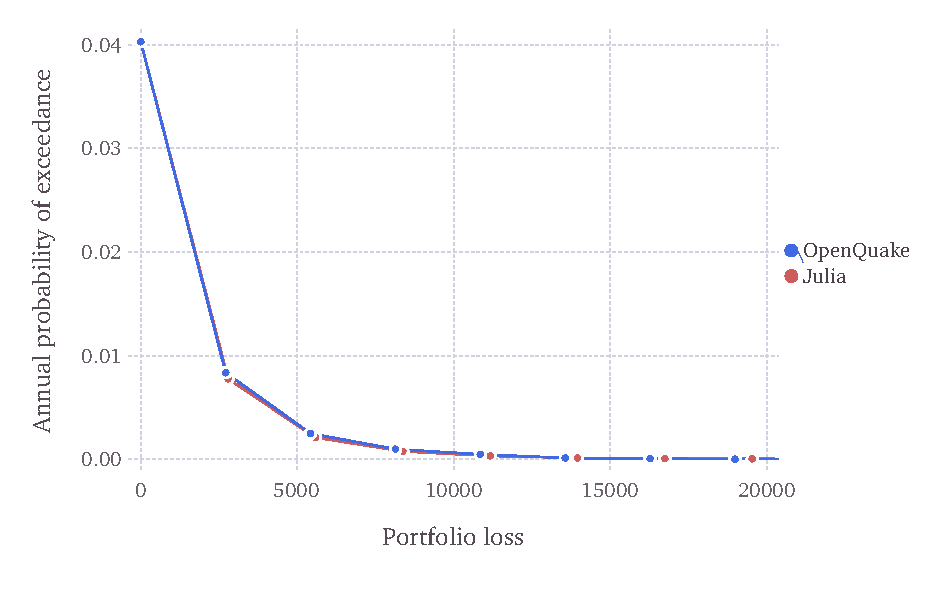
\includegraphics[width=12cm]{qareport/figures/fig-lc-ebr-6c}
\caption{Portfolio loss curve comparison for event based risk test case 6c}
\label{fig:lc-ebr-6c}
\end{figure}
\begin{table}[htbp]

\centering
\begin{tabular}{ l l r r r }

\hline
\rowcolor{anti-flashwhite}
\bf{Asset} & \bf{Result} & \bf{Julia} & \bf{OpenQuake} & \bf{Difference}\\
\hline
Portfolio & Average loss & 87.61 & 88.61 & 1.13\% \\
\hline
\end{tabular}

\caption{Results for event based risk test case 6c}
\label{tab:result-ebr-6c}
\end{table}
Table \ref{tab:result-ebr-6c} shows the comparison of the OpenQuake result for average portfolio loss with the expected result.

% ---------------------------------------------------------------------------
\subsubsection{Case 6d}
This case is designed to test the computation of the individual asset loss curves, the portfolio loss exceedance curve, average asset losses, and the average portfolio loss, when the vulnerability models of different assets of the same taxonomy are treated as partially correlated, with a coefficient of correlation of $0.5$. In OpenQuake, this can be specified in the job configuration file, by setting the value of the parameter `asset\_correlation' to $0.5$.

The list of assets and their taxonomies are shown in Table~\ref{tab:assets-tax1}. Table~\ref{tab:vf-ln-tax3-zcov} shows the mean loss ratios and corresponding coefficients of variation in the vulnerability function used in this test case. Ground motion fields are generated for each of the ruptures generated in the 100,000 stochastic event sets as described in Case~6a and Case~6b. These ground motion fields are also used for the corresponding calculation in Julia.

Since the sampled loss ratios conditional on a given ground motion field for different assets of the same taxonomy are assumed to be  correlated in this case, we proceed by first generating a vector of \emph{epsilons} for each taxonomy from the multivariate standard normal distribution which has the symmetric covariance matrix with $1.0$ as the diagonal elements and $\rho = 0.5$ as the off-diagonal elements.

Now, for each asset of that taxonomy, the parameters $m$ and $s$ are obtained for the ground motion value at the location of the asset through interpolation on the specified vulnerability model. Each asset of a particular taxonomy is also assigned a value of $\epsilon$ from the vector of \emph{epsilons} for that taxonomy sampled as described above. The parameters $m$ and $s$ are then converted to the parameters $\mu$ and $\sigma$ of the corresponding normal distribution, and the sampled loss ratio is obtained simply as $\exp (\mu + \epsilon * \sigma)$.

After the asset event loss tables are compiled by sampling correlated loss values as described above, the rest of the calculation concerning the derivation of asset and portfolio loss curves and average asset and portfolio loss proceeds as in previous cases. The portfolio loss curve calculated using the implementation of the calculator in Julia is compared with that produced by OpenQuake in Figure~\ref{fig:lc-ebr-6d}. Only the aggregated results for the portfolio are shown here for brevity.

\begin{figure}[htbp]
\centering
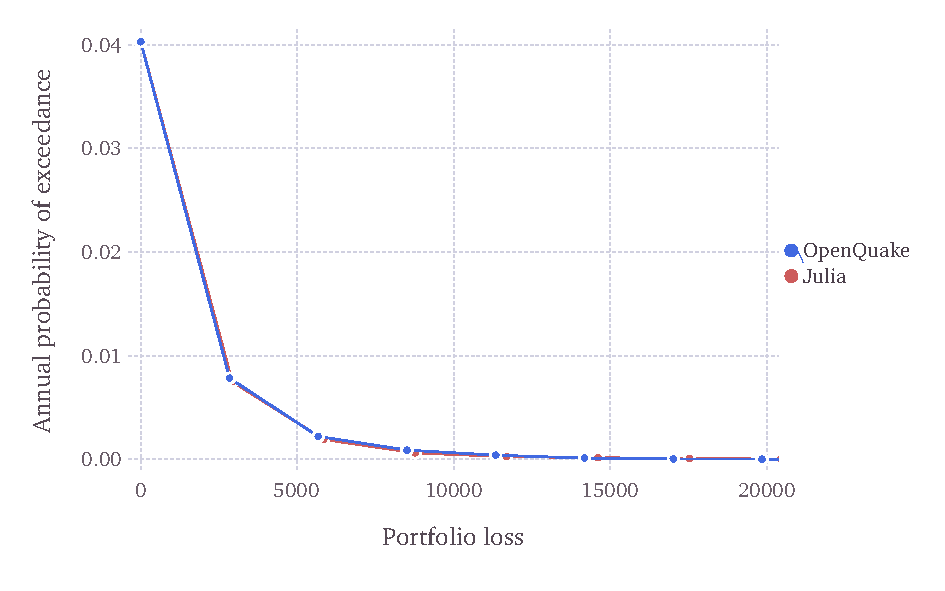
\includegraphics[width=12cm]{qareport/figures/fig-lc-ebr-6d}
\caption{Portfolio loss curve comparison for event based risk test case 6d}
\label{fig:lc-ebr-6d}
\end{figure}
\begin{table}[htbp]

\centering
\begin{tabular}{ l l r r r }

\hline
\rowcolor{anti-flashwhite}
\bf{Asset} & \bf{Result} & \bf{Julia} & \bf{OpenQuake} & \bf{Difference}\\
\hline
Portfolio & Average loss & 89.72 & 89.76 & 0.05\% \\
\hline
\end{tabular}

\caption{Results for event based risk test case 6d}
\label{tab:result-ebr-6d}
\end{table}
Table \ref{tab:result-ebr-6d} shows the comparison of the OpenQuake result for average portfolio loss with the expected result.

% ---------------------------------------------------------------------------